%%%%%%%%%%%%%%%%%%%%%%%%%%%%%%%%%%%%%%%%%
% Arsclassica Article
% LaTeX Template
% Version 1.1 (10/6/14)
%
% This template has been downloaded from:
% http://www.LaTeXTemplates.com
%
% Original author:
% Lorenzo Pantieri (http://www.lorenzopantieri.net) with extensive modifications by:
% Vel (vel@latextemplates.com)
%
% License:
% CC BY-NC-SA 3.0 (http://creativecommons.org/licenses/by-nc-sa/3.0/)
%
%%%%%%%%%%%%%%%%%%%%%%%%%%%%%%%%%%%%%%%%%

%----------------------------------------------------------------------------------------
%	PACKAGES AND OTHER DOCUMENT CONFIGURATIONS
%----------------------------------------------------------------------------------------

\documentclass[
12pt, % Main document font size
a4paper, % Paper type, use 'letterpaper' for US Letter paper
oneside, % One page layout (no page indentation)
%twoside, % Two page layout (page indentation for binding and different headers)
headinclude,footinclude, % Extra spacing for the header and footer
BCOR5mm, % Binding correction
]{scrartcl}

%%%%%%%%%%%%%%%%%%%%%%%%%%%%%%%%%%%%%%%%%
% Arsclassica Article
% Structure Specification File
%
% This file has been downloaded from:
% http://www.LaTeXTemplates.com
%
% Original author:
% Lorenzo Pantieri (http://www.lorenzopantieri.net) with extensive modifications by:
% Vel (vel@latextemplates.com)
%
% License:
% CC BY-NC-SA 3.0 (http://creativecommons.org/licenses/by-nc-sa/3.0/)
%
%%%%%%%%%%%%%%%%%%%%%%%%%%%%%%%%%%%%%%%%%

%----------------------------------------------------------------------------------------
%	REQUIRED PACKAGES
%----------------------------------------------------------------------------------------

\usepackage[
nochapters, % Turn off chapters since this is an article        
beramono, % Use the Bera Mono font for monospaced text (\texttt)
eulermath,% Use the Euler font for mathematics
pdfspacing, % Makes use of pdftex’ letter spacing capabilities via the microtype package
dottedtoc % Dotted lines leading to the page numbers in the table of contents
]{classicthesis} % The layout is based on the Classic Thesis style

\usepackage{arsclassica} % Modifies the Classic Thesis package

\usepackage[T1]{fontenc} % Use 8-bit encoding that has 256 glyphs

\usepackage[utf8]{inputenc} % Required for including letters with accents

\usepackage{graphicx} % Required for including images
\graphicspath{{Figures/}} % Set the default folder for images

\usepackage{enumitem} % Required for manipulating the whitespace between and within lists

\usepackage{lipsum} % Used for inserting dummy 'Lorem ipsum' text into the template

\usepackage{subfig} % Required for creating figures with multiple parts (subfigures)

\usepackage{amsmath,amssymb,amsthm} % For including math equations, theorems, symbols, etc

\usepackage{varioref} % More descriptive referencing

%----------------------------------------------------------------------------------------
%	THEOREM STYLES
%---------------------------------------------------------------------------------------

\theoremstyle{definition} % Define theorem styles here based on the definition style (used for definitions and examples)
\newtheorem{definition}{Definition}

\theoremstyle{plain} % Define theorem styles here based on the plain style (used for theorems, lemmas, propositions)
\newtheorem{theorem}{Theorem}

\theoremstyle{remark} % Define theorem styles here based on the remark style (used for remarks and notes)

%----------------------------------------------------------------------------------------
%	HYPERLINKS
%---------------------------------------------------------------------------------------

\hypersetup{
%draft, % Uncomment to remove all links (useful for printing in black and white)
colorlinks=true, breaklinks=true, bookmarks=true,bookmarksnumbered,
urlcolor=webbrown, linkcolor=RoyalBlue, citecolor=webgreen, % Link colors
pdftitle={}, % PDF title
pdfauthor={\textcopyright}, % PDF Author
pdfsubject={}, % PDF Subject
pdfkeywords={}, % PDF Keywords
pdfcreator={pdfLaTeX}, % PDF Creator
pdfproducer={LaTeX with hyperref and ClassicThesis} % PDF producer
} % Include the structure.tex file which specified the document structure and layout

\usepackage{geometry}
\usepackage{float}

\hyphenation{Fortran hy-phen-ation e-ser-ci-ta-zio-ne} % Specify custom hyphenation points in words with dashes where you would like hyphenation to occur, or alternatively, don't put any dashes in a word to stop hyphenation altogether

%----------------------------------------------------------------------------------------
%	TITLE AND AUTHOR(S)
%----------------------------------------------------------------------------------------

\title{\normalfont\spacedallcaps{Relazione MEMOC}} % The article title

\author{\spacedlowsmallcaps{Giulio Lovisotto - 1084847} \\ \normalsize{\spacedallcaps{Universita' degli studi di Padova}}} % The article author(s) - author affiliations need to be specified in the AUTHOR AFFILIATIONS block

\date{16 Settembre 2015} % An optional date to appear under the author(s)

%----------------------------------------------------------------------------------------

\begin{document}

%----------------------------------------------------------------------------------------
%	HEADERS
%----------------------------------------------------------------------------------------

\renewcommand{\sectionmark}[1]{\markright{\spacedlowsmallcaps{#1}}} % The header for all pages (oneside) or for even pages (twoside)
%\renewcommand{\subsectionmark}[1]{\markright{\thesubsection~#1}} % Uncomment when using the twoside option - this modifies the header on odd pages
\lehead{\mbox{\llap{\small\thepage\kern1em\color{halfgray} \vline}\color{halfgray}\hspace{0.5em}\rightmark\hfil}} % The header style

\pagestyle{scrheadings} % Enable the headers specified in this block

%----------------------------------------------------------------------------------------
%	TABLE OF CONTENTS & LISTS OF FIGURES AND TABLES
%----------------------------------------------------------------------------------------

\maketitle % Print the title/author/date block

\setcounter{tocdepth}{2} % Set the depth of the table of contents to show sections and subsections only

%\tableofcontents % Print the table of contents

%\listoffigures % Print the list of figures

%\listoftables % Print the list of tables

%----------------------------------------------------------------------------------------
%	ABSTRACT
%----------------------------------------------------------------------------------------

%\section*{Abstract} % This section will not appear in the table of contents due to the star (\section*)

% \lipsum[1] % Dummy text

%----------------------------------------------------------------------------------------
%	AUTHOR AFFILIATIONS
%----------------------------------------------------------------------------------------

%{\let\thefootnote\relax\footnotetext{* \textit{Department of Biology, University of Examples, London, United Kingdom}}}

%{\let\thefootnote\relax\footnotetext{\textsuperscript{1} \textit{Department of Chemistry, University of Examples, London, United Kingdom}}}

%----------------------------------------------------------------------------------------

%\newpage % Start the article content on the second page, remove this if you have a longer abstract that goes onto the second page

%----------------------------------------------------------------------------------------
%	INTRODUCTION
%----------------------------------------------------------------------------------------

\section{Introduzione}

Questo documento descrive le metodologie e le strutture sviluppate per l'esercitazione del corso di Metodi e Modelli per l'Ottimizzazione combinatoria, anno accademico 14/15. L'esercitazione consiste nella risoluzione del  Traveling Salesman Problem (TSP) con l'uso di metodi di ottimizzazione. E' stato implementato il modello per il risolutore esatto \textsc{cplex}, e una metaeuristica di tipo particle swarm optimization \textsc{pso}. Il seguente documento e' strutturato come segue: in Sezione~\ref{sec:cplex} viene descritto il modello in \textsc{cplex} (relativo alla Parte 1), in Sezione~\ref{sec:eur} vengono descritte le euristiche utilizzate (relative allla Parte 2), in Sezione~\ref{sec:exp} vengono descritti i dataset e la metodologia usata per l'esperimento, nonche' presentati i risultati. Il documento termina con alcune conclusioni in Sezione~\ref{sec:conclusioni}.

\subsection{FILES CONSEGNATI}

\begin{itemize}
\item something;
\item something else.
\end{itemize}

\section{Modello CPLEX} \label{sec:cplex}

In questa sezione viene descritto in che modo e' stato realizzato il modello per TSP che viene usato per la risoluzione con \textsc{cplex}. Per realizzare tale modello e' stata utilizzata la formalizzazione del TSP fornita dal docente~\cite{luigitraccia1}. Tale formalizzazione modella il problema come un problema di ottimizzazione su reti di flusso. E' stato realizzato un unico file \texttt{cplex.cpp}. Esso procede secondo i seguenti passi:
\begin{enumerate}
 \item legge il problema in input, che consiste in un file di testo riportante la matrice contenente i costi degli archi del grafo (separati da virgole), e inizializza le variabili del problema e la funzione obiettivo, impostando i vincoli di tipo e i bounds per ciascuna variabile;
 \item per ogni vincolo, lo crea e lo aggiunge alla matrice dei coefficienti dell'istanza del problema. Le variabili relative ai cappi (cioe' $x_{ii}, y_{ii}$) vengono rimosse;
 \item esegue l'ottimizzazione e salva i risultati su file, tra i quali tempo di esecuzione, path ottimo, costo della soluzione ottima trovata.
\end{enumerate}

%----------------------------------------------------------------------------------------
%	RESULTS AND DISCUSSION
%----------------------------------------------------------------------------------------

\section{Metaeuristiche} \label{sec:eur}
In questa sezione vengono descritte le metaeuristiche implementate per la risoluzione di TSP. 

\subsection{Particle Swarm Optimization}

\textsc{pso} e' una metaeuristica basata su popolazione. In esso, gli individui $x_k$ (possibili soluzioni) si muovono nello spazio N-dimensionale secondo le loro rispettive velocita' $v_k$. In \textsc{pso} gli individui ricordano la miglior posizione da loro visitata, e la miglior posizione globale visitata dalla popolazione. Tali posizioni influiscono sulla velocita' dell'iterazione successiva. 

Per applicare tale metodo a TSP e' necessario renderlo discreto. E' stata scelta la rappresentazione proposta in~\cite{1259748} e ripresa in~\cite{shi2007particle}. In essa, gli individui sono cicli sul grafo che rappresenta il problema, e le velocita' sono sequenze di ``Swap Operator''. Uno Swap Operator (SO) e' definito da una coppia $(i, j)$, la sua applicazione su una soluzione $x_k$ ha l'effetto di scambiare la componente $i$-esima con la componente $j$-esima. E' importante notare che dato che le soluzioni $x_k$ sono cicli sul grafo, l'applicazione di uno SO ad una soluzione $x_k$ genera una nuova soluzione valida. Per formalizzare la rappresentazione  e' necessario introdurre 4 operatori:
\begin{itemize}
\item $x + v,$ dove $x$ e' una possibile soluzione e $v$ e' una sequenza di SO. Ottiene una nuova soluzione applicando gli SO in $v$ alla soluzione $x$;
\item $v_1 \otimes v_2,$ dove $v_1, v_2$ sono sequenze di SO. Produce la piu' corta sequenza di SO il cui effetto e' equivalente all'applicazione di $v_1$ e $v_2$ in successione;
\item $x-y,$ dove $x, y$ sono possibili soluzioni. Produce la piu' corta sequenza di SO che applicata a $y$ (con l'operatore $+$) ritorna $x$;
\item $a * v,$ dove $a$ e' uno scalare, e $v$ e' una sequenza di SO. Produce una nuova sequenza di SO a partire da $v$ rimuovendo con probabilita' $1-a$ ogni suo SO.
\end{itemize}
La regola di aggiornamento delle velocita' per il generico individuo $k$ all'iterazione $i$-esima e' la seguente:

\[ v^{(i+1)}_k = v_k^{(i)} \otimes \alpha \ast (p_k^{(i)} - x_k) \otimes \beta \ast (g^{(i)} - x_k) \quad \alpha, \beta \in [0, 1], \]

dove $p_k^{(i)}$ e' la miglior soluzione visitata dall'individuo $k$, e $g^{(i)}$ e' la miglior soluzione visitata dalla popolazione, finora. Alla fine dell'iterazione $i$-esima l'individuo $x_k$ si trova in posizione $x_k + v_k^{(i)}$. Ad ogni iterazione ogni individuo viene valutato e le miglior soluzioni visitate vengono aggiornate.

E' stato realizzato un singolo file \texttt{pso.cpp}. Gli individui sono rappresentati da array di interi (\texttt{vector<int>}), dove ogni elemento fa riferimento ad un nodo del problema. Gli SO sono coppie di interi, le velocita' (sequenze di SO) sono array di coppie di interi (\texttt{vector<pair<int, int> >}). Gli operatori introdotti precedentemente in questo paragrafo sono realizzati tramite funzioni. Il file legge il problema in input (nel formato riportato in Sezione~\ref{sec:cplex}). La popolazione e' inizializzata con individui random, le velocita' iniziali sono sequenze di SO di lunghezza random tra 0 ed $N$ (numero di nodi). Gli elementi su cui effettuare swap sono scelti in maniera random. Viene eseguita l'ottimizzazione e vengono salvati i risultati su file.

\section{Esperimenti}\label{sec:exp}
In questa sezione vengono riportate le tecniche utilizzate per generare i dataset, le metodologie usate per gli esperimenti, e i risultati ottenuti.

\subsection{Dataset}
I dataset consistono in insiemi di $n$ punti, $n \in \{9, 16, 25, 36, 49, 64\}$, distribuiti un quadrato bidimensionale con lato di dimensione 1. Sono stati usati 3 diversi criteri per la disposizione dei punti:
\begin{itemize}
	\item \textbf{random} i punti sono scelte in maniera casuale;
	\item \textbf{uniform} i punti sono disposti a formare una griglia;
	\item \textbf{clustered} viene creato un grafo, e viene disegnato con l'utility \textsc{dot}~\cite{gansner2006drawing}. Le coordinate dei nodi nel layout ottenuto sono le posizioni dei punti.
\end{itemize}
Per i dataset con criterio \textbf{random} e \textbf{clustered} vengono generate 20 istanze per ogni dimensione. Figure \ref{fig:rnd} e \ref{fig:cls} riportano degli esempi di istanza per questi layout. 

\begin{figure}[H]
	\centering
	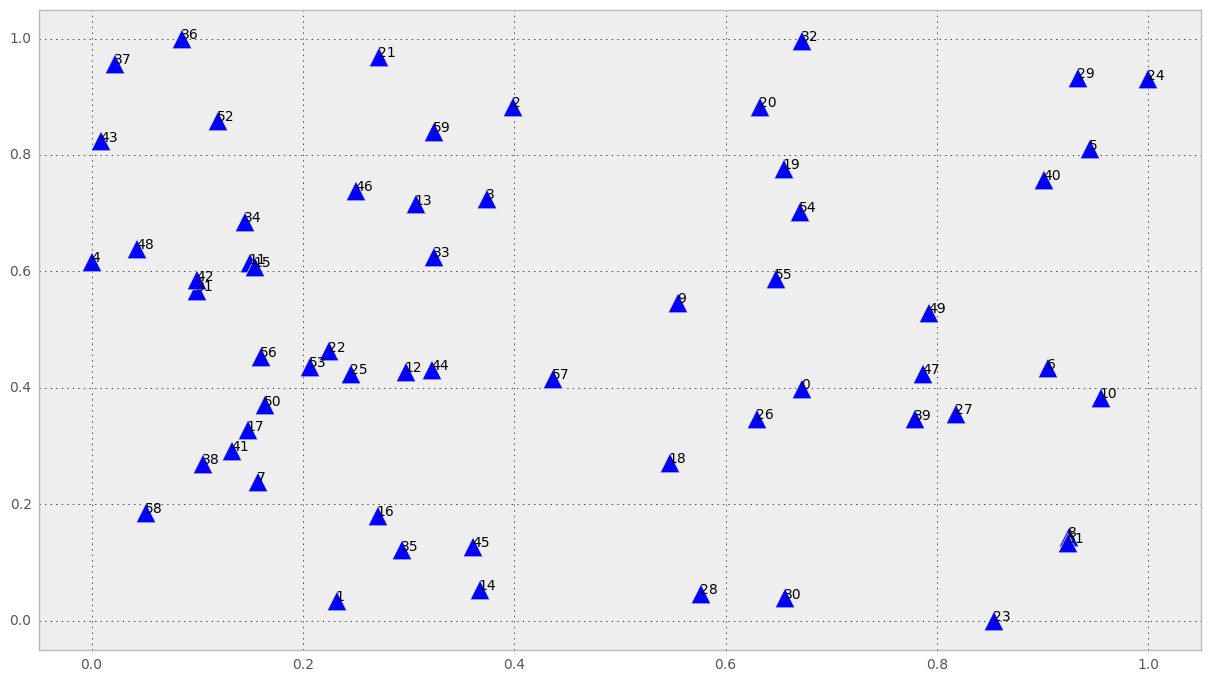
\includegraphics[width=.9\columnwidth]{rnd_example}
	\caption[random]{Esempio di dataset con layout random.}
	\label{fig:rnd}
\end{figure}

\begin{figure}[H]
	\centering
	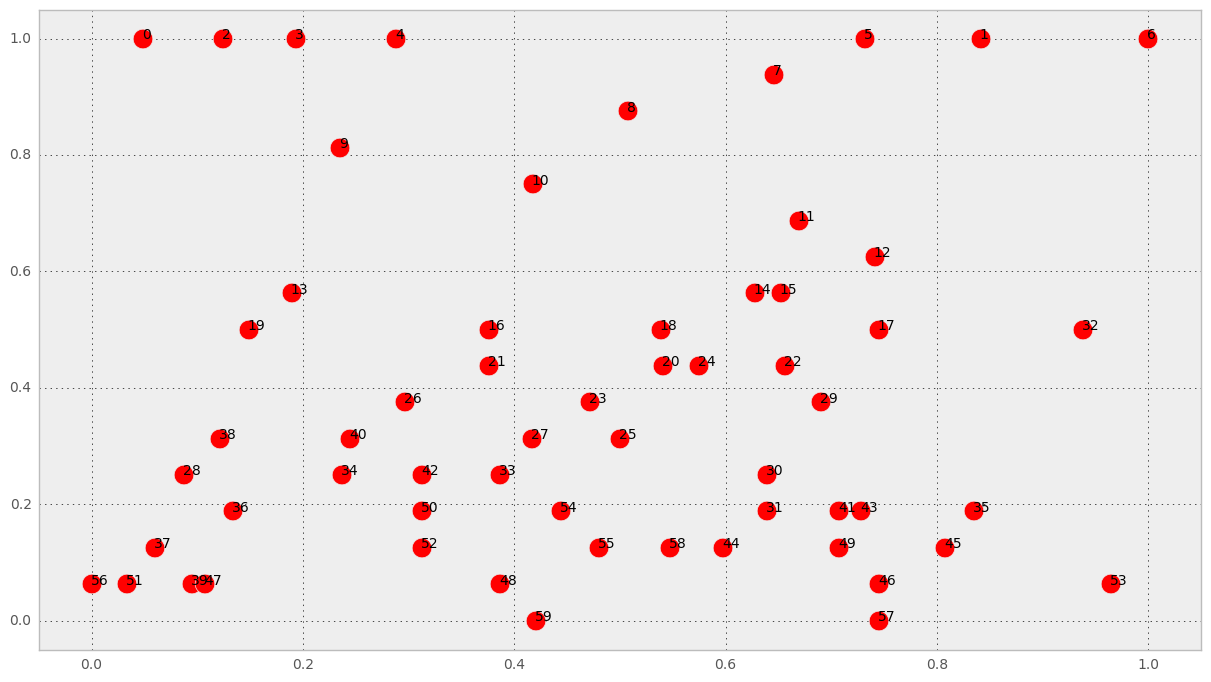
\includegraphics[width=.9\columnwidth]{cls_example}
	\caption[clustered]{Esempio di dataset con layout clustered.}
	\label{fig:cls}
\end{figure}

\subsection{Metodologia e Parametri}

Gli esperimenti sono stati svolti su macchine cosicosi. Essi consistono nell'utilizzare le tecniche descritte in Sezione \ref{sec:cplex} e \ref{sec:eur} per risolvere il TSP, sui dataset generati. Per ogni dataset, ogni risolutore viene eseguito 5 volte, e vengono salvate le medie e le standard deviation dei tempi di esecuzione e dei costi delle soluzioni ottime trovate. 

Per \textsc{pso} e' stata utilizzata una popolazione di 2.000 individui, 1.000 iterazioni, $\alpha = 0.75$, $\beta=0.1$ (i parametri sono stati scelti empiricamente, senza un estensivo procedimento di ottimizzazione).


\subsection{Risultati}
plotsplotsplots
Potrebbe essere interessante vedere in percentuale quanti degli archi usati da pso sono parte dell'ottimo. Interessante vedere fevals durante pso.
\section{Conclusioni}\label{sec:conclusioni}

%----------------------------------------------------------------------------------------
%	BIBLIOGRAPHY
%----------------------------------------------------------------------------------------

\renewcommand{\refname}{\spacedlowsmallcaps{References}} % For modifying the bibliography heading

\bibliographystyle{unsrt}

\bibliography{bibliography.bib} % The file containing the bibliography

%----------------------------------------------------------------------------------------

\end{document}
